\documentclass[10pt,a4paper,final,oneside,openany]{memoir}

\usepackage[english]{babel}
\usepackage[utf8]{inputenc}
\usepackage[T1]{fontenc}
\usepackage[british]{isodate}

% Layout Fixes
\usepackage{booktabs} % nicer spacing between table rulers
\usepackage{microtype}
\usepackage{fixltx2e} % To prevent the figures from being placed
                      % out-of-order with respect to their
                      % "non-starred" counterparts


\usepackage{amsmath,amssymb, amsbsy}
\usepackage[amsmath,amsthm,thmmarks]{ntheorem}
\usepackage{semantic, stmaryrd}
\usepackage{graphicx}
\usepackage[disable]{todonotes}
\presetkeys{todonotes}{inline}{}
\usepackage{adjustbox}
\usepackage{tikz}
\usetikzlibrary{trees}
\usepackage{algpseudocode}
\usepackage{algorithm}
\usepackage{listings}
\usepackage{pdfpages}

\lstset{basicstyle=\footnotesize\ttfamily,breaklines=true, language=Haskell}

% ADD "parfor" to algorithmic environment
  % declaration of the new block
  \algblock{ParFor}{EndParFor}
  % customising the new block
  \algnewcommand\algorithmicparfor{\textbf{parfor}}
  \algnewcommand\algorithmicpardo{\textbf{do}}
  \algnewcommand\algorithmicendparfor{\textbf{end\ parfor}}
  \algrenewtext{ParFor}[1]{\algorithmicparfor\ #1\ \algorithmicpardo}
  \algrenewtext{EndParFor}{\algorithmicendparfor}

% Bibliography
%\usepackage[style=alphabetic,natbib=true]{biblatex}
\usepackage[hyperref,style=numeric,natbib=true, defernumbers=true]{biblatex}
\usepackage[hyperindex,hidelinks]{hyperref}

% Fonts
\usepackage{palatino}
\linespread{1.05}
\usepackage[scaled]{beramono}

% customize chapter pages
\makepagestyle{myheadings}
\makepagestyle{myheadingschapterpage}
\makeevenfoot{myheadingschapterpage}{}{\thepage}{}
\makeoddfoot{myheadingschapterpage}{}{\thepage}{}
\aliaspagestyle{chapter}{myheadingschapterpage}
\aliaspagestyle{title}{myheadingschapterpage}
\makeevenhead{myheadings}{}{\scshape \thetitle}{}
\makeoddhead{myheadings}{}{\footnotesize\scshape \thetitle}{}
\makeevenfoot{myheadings}{}{\thepage}{}
\makeoddfoot{myheadings}{}{\thepage}{}
\pagestyle{myheadings}

\def\thefigure{\arabic{figure}}
\setcounter{tocdepth}{0}


\setcounter{secnumdepth}{1}
\setcounter{chapter}{0}
\setsecheadstyle{\large\bfseries\raggedright}
\setsubsecheadstyle{\bfseries}

% BIBLIOGRAPHY styling
% Print the DOI url out
%\newcommand*{\doi}[1]{DOI: \url{http://dx.doi.org/#1}}

\DeclareFieldFormat{doi}{\textsc{doi}: \url{http://dx.doi.org/#1}}
\DeclareNameAlias{default}{last-first/first-last}
%\DeclareFieldFormat{title}{\emph{#1}}
\renewcommand\mkbibnamefirst[1]{\textsc{#1}}
\renewcommand\mkbibnamelast[1]{\textsc{#1}}
\renewcommand*{\bibfont}{\footnotesize}

% No page numbers for parts in TOC
\cftpagenumbersoff{part}
% Footnote symbols
%\renewcommand*{\thefootnote}{\fnsymbol{footnote}}

% Figures
\newsubfloat{figure}

\usepackage{sidecap}
\usepackage{caption}
\captionsetup{margin=0pt, font=small, labelfont=bf, format=hang}
\setlength{\abovecaptionskip}{0pt}
\setlength{\belowcaptionskip}{0pt}


% Default commands
\newcommand{\subimgwidth}{.48\textwidth}
\newcommand{\imgwidth}{.85\textwidth}


\newtheorem{example}{Example}
%
\theoremstyle{plain}
\theoremsymbol{\tiny $\Box$}
\newtheorem{definition}[equation]{Definition}


% Bitwise and and or operators
% http://tex.stackexchange.com/questions/39313/double-nested-logical-and-and-logical-or-symbols
\DeclareFontFamily{U}{matha}{\hyphenchar\font45}
\DeclareFontShape{U}{matha}{m}{n}{
      <5> <6> <7> <8> <9> <10> gen * matha
      <10.95> matha10 <12> <14.4> <17.28> <20.74> <24.88> matha12
      }{}

\newcommand{\bland}{\mathbin{
  \raisebox{.1ex}{%
    \rotatebox[origin=c]{-90}{\usefont{U}{matha}{m}{n}\symbol{\string"CE}}}}}
\newcommand{\blor}{\mathbin{
  \raisebox{.1ex}{%
    \rotatebox[origin=c]{90}{\usefont{U}{matha}{m}{n}\symbol{\string"CE}}}}}



%%% Local Variables: 
%%% mode: latex
%%% TeX-master: "master"
%%% End: 


\title{Applying data-parallel languages to option pricing}
\author{
  Martin Dybdal -- \texttt{dybber@dybber.dk} \\
  Philip Carlsen -- \texttt{plcplc@gmail.com}
\\
University of Copenhagen, DIKU}

\date{\today}

\bibliography{../bibliography/bibliography}

\begin{document}
\maketitle
\begin{abstract}
Here goes the abstract
\end{abstract}

\newpage
\renewcommand*{\cftpartname}{Part\space}
%\renewcommand*{\cftchaptername}{Chapter\space}
%\renewcommand{\cftchapterindent}{1em}
\tableofcontents*

\chapter{Preface}
This dissertation is submitted in fulfillment of the graduate education
in computer science (\textit{Datalogi}) at the University of
Copenhagen, for Philip L. Carlsen and Martin Dybdal. In addition, the
dissertation also serves as partial fulfillment of Martin Dybdal's 4+4
Ph.D. education at the University of Copenhagen.

The thesis has been supervised by Ken Friis Larsen and we would like
to thank him for valuable supervision hours .... We would also like to
thank Geoffrey Mainland and Trevor McDonell for valuable email
correspondences and quick responses in cases of problems with their
libraries... Finally we would like to thank Cosmin Oancea, Christian
Andretta, Jost Berthold, Martin Elsman and others here at the HIPERFIT
research center.

% Disposition for introduction:
% \begin{itemize}
% \item Where does performance and programmer efficiency come from
% \item The free lunch is over
% \item (Embarassingly parallel problems)
% \item Why the language-based approach?
% \item Parallel Functional Programming
% \item What is a "vector language"?
% \item Our strategy: implement real world example applications, study
%   limitations of current approaches, extend and modify until we get
%   better results.
% \item Report Outline
% \end{itemize}

\chapter{Introduction}
\section{Background}
Ever since the first electronic computers were built, there has been a
wish for tackling larger and more complex problems, which in turn has
created an increasing demand for performance improvements and
increased programmer productivity. Performance improvements originate
from improvements in either hardware or the employed
algorithms. Programmer productivity, on the other hand, correlates
with the features of the used programming language and programming
environment (IDEs, debuggers, etc.). A language providing high
programmer efficiency should make it easy to implement and reason
about algorithms, make mistakes easily avoidable and when a mistake
happens, make it easy to uncover its cause.

For a handful of decades, we have been able to increase performance
through hardware improvements of sequential processors and we have
thus been able to stick with more or less the same model of
computation. Recently, hardware developers have faced physical
barriers, making further performance improvements of sequential
processors impractical, and they have had to go new ways to obtain the
desired speed-up \cite{sutter2006freelunchisover}. These new
architectures call for new algorithms and models of computation, as
well as new languages and programming tools to keep the complexity of
software development at a tolerable level.

We will focus on software development for \emph{graphics processing
  units} (GPUs), which in recent years have been found cost-effective
alternatives to ordinary CPUs, for many other domains than computer
graphics. Today they are employed in fields as diverse as
bioinformatics, computational chemistry, medical image analysis,
relational databases, computational finance and simulation in both
engineering and the sciences \cite{hwy2011emerald, hwu2011jade,
  owens2007survey}. Solutions to many problems in these domains can be
expressed naturally as \emph{data-parallel} algorithms, where each
data item can be processed independently (often from a linear algebra
specification of the problem). This is thus where GPUs popularity
arise; executing such data-parallel tasks is the core capability of
GPUs.

% Should we include this somewhere?
% GPUs have gained so much popularity that they are a main ingredient in
% quite a few of todays largest supercomputers \cite{Top500}.

\section{Data-parallel programming languages}
Even though we think of graphics processors as \emph{modern
  hardware}, the software development tools in widespread use for
programming them are far from modern. CUDA
\cite{nvidia2012programming} and OpenCL \cite{munshi2011opencl}, the
two main languages for programming GPUs are low-level languages with
manual memory management, limited abstractions, and tedious hand
optimization are often required. It is, for instance, important to
streamline memory accesses to get decent performance. The low-level
nature of these languages makes automated code analysis difficult. The
NVIDIA CUDA compiler thus cannot make an optimization such as stream
fusion (deforestation), that removes intermediate data structures and
thus removes the need for very costly memory transactions. The
programmer thus has to fuse programs by hand, sacrificing clarity as
abstractions between individual parts has to be broken down and fused
together. Also, the programmer has to be well aware of the exact
hardware his program is to be executed on, thus making a tight
coupling between program and hardware.

High-level languages for GPU programming have been developed and
employed, but none of them have found as widespread use as programming
directly in CUDA or OpenCL. These newer languages include
Theano\cite{bergstra2010theano},
Accelerate\cite{chakravarty2011accelerating},
Nikola\cite{mainland2010nikola}, Obsidian\cite{svensson2011obsidian},
Intel Array Building Blocks \cite{newburn2011intel}, Bohrium
\cite{homepage:bohrium} and Copperhead \cite{Catanzaro2011}. Their
common aim is to abstract away the underlying hardware platform and
let data-parallel problems be easily specified.

These languages share the characteristica of lifting operations to
work collectively on vectors rather than individually on primitive
values (such as integers and floating point number).

We want to join in and contribute to these languages, and we believe
that such an endeavour should start with evaluating current state of
the art, such that we can make sure our contributions will be relevant
and beneficial. Thus, the first part of this report is a survey of
some of the existing parallel functional programming languages. We
have taken the strategy of implementing some real world example
applications from the financial domain, to study the limitations of
current approaches.

% \todo{Add note on mapping nested data-parallelism to flat
%   architectures is still an open problem, as vectorisation is not the
%   holy grail}

\section{Contributions}

We have conducted a small survey comparing a few Haskell libraries and
languages with respect to their performance, expressivity and the apparent
health of their supporting project's infrastructure.

Taking an outset in two common financial algorithms for option pricing
and a quasi-random number generator, we have found that the lack of
nesting in a language such as Accelerate and Nikola is too limiting to
implement concise solutions and that the specification of some
algorithms would lead to incomposable constructs.

As this lack of nesting is due to excessive and concious limitation,
we suggest taking a step back and give the programmer more control,
though giving away some of the guarantees made by a strict type system
of performance and absolute correctness. Of our surveyed languages,
Nikola fits this view the best, and is selected as the subject for
further study.

This we go about by exploring the implementation of a few but
motivated extra array operators, and last we present a proposal to
deal with the problem posed by mapping nested array
operators\footnote{We avoid the term nested data-parallelism, as that
  is often connotated with the vectorisation transformation} to flat
parallel hardware. This proposal uses a cursor to mark the limit
between sequential and parallel code, and we find at promising
alternative to vectorisation. There is a large body of future work in
deducing the consequences of such a language addition.

% \begin{itemize}

% \item A survey comparing of the vector languages CUDA, R, Repa, Accelerate and
%   Nikola. The comparison is based on how well they performed with our cases,
%   both in terms of expressivity and performance, and the surrounding community
%   of developers and users.

% \item We found Nikola to be the most promising candidate for useful extensions.

% \item We have implemented prototypes of folding, unfolding and nested maps in
%   Nikola. While there is yet some way to an acceptable implementation, we
%   outline a way to it.

% \item We present an alternative way of expressing nested data parallelism, that
%   doesn't involve an elaborate code transformation like \cite{nesl}, and
%   doesn't impair the compositionality of the language. Like above, we have yet
%   to actually test the method in practise.

% \end{itemize}

%
%* Example where the Accelerate breaks down, and code does not seem to
%  be written clearly
%
%* An alternative approach to specifying

All the source code associated with the practical execution of the survey, as well as this report is hosted at
\url{https://github.com/HIPERFIT/vectorprogramming/}.
The extensions developed for Nikola are to be found at \url{https://github.com/HIPERFIT/nikola/}.

\section{Report outline}
The remainder of the report is structured as follows. This
introductory chapter is supplemented with two chapters introducing
terminology: one on hardware platforms such as GPUs and one on the
financial example problems we are going to use throughout the
report.

The rest of the report after these introductory chapters is divided
into two more or less independent parts. The first part contains a
survey of currently used data-parallel languages. The second part
describes our own efforts into extending the GPU language Nikola with
functionality we found lacking in the experiments conducted throughout
the survey.

% \todo{Use refs to chapters and parts in outline}

%%% Local Variables:
%%% mode: latex
%%% TeX-master: "master"
%%% End:

\chapter{Cases}
\label{chap:cases}

In this chapter we will introduce the cases which we will use as
benchmarks in our survey and as offset for our extensions of the
Nikola language. All cases are drawn from the financial domain and the
affiliated domain of scientific computing.

\section{Option pricing}
Finance as a mathematical discipline is concerned with the pricing of
assets.  Financial assets can be material objects such as goods, or
contracts on other assets. The \emph{stock} issued by a company is a
common example of a financial contract. However, as this definition of
a financial asset is recursive, contracts on other contracts are
possible. An \emph{option} to buy or sell some other asset for some
price at some point in time is a common example, and the one that we
will invest some of our effort treating. These types of contracts are
commonly termed \emph{financial derivatives}.

\emph{Option} is the name used collectively for a range of different
financial contracts that all share some features, namely that an
option on an underlying asset $A$ gives the holder the right to
exchange $A$ for a certain strike price $K$ in a certain time interval
up until a prespecified expiration time $T$.

The different types of options vary the processes that determine the
size of strike price and the time span where the option may be
exercised.  We make a distinction between options that grants a right
to buy and those that grants a right to sell. A \emph{call option} on
asset $A$ grants the right to buy $A$, whereas a \emph{put option}
grants the right to sell.

For a concrete example, consider this:
\begin{example}[European Call Option]
  European options\footnote{The continent of Europe is completely unrelated to
  the naming of this contract.} are characterised by having a pre-determined
  constant strike price $K$, and may be exercised only on the expiration time
  $T$.

  \begin{itemize}
  \item Assume the price of a stock $A$ is quoted as $S_0=\$90$ at time
    $t_0$, and that an European call option for the stock has a strike
    price of $K=\$100$ and expiration time $T=t_1$.

    % \item So, having acquired a European call option for 1 of IBM company stock
    %   with strike price \$100 and expiration time January 1st, we wait.
    %   \todo{What is $S_0$ in this example?}

  \item When upon the arrival of $t_1$ we observe that $A$ is now
    exchanged at value $S_1=\$105$, we choose to exercise our option right
    and thus recieve 1 stock for \$100.

    \item Immediately, we sell this stock on the market for \$105 and have thus
      earned $S_1-K=\$5$. Our option was ``in the money''.
  \end{itemize}

  Note that in reality, the underlying asset rarely changes hands. Instead,
  only the net difference in strike price and market price is
  exchanged.\footnote{A consequence of this is that you are not required to
  actually own any quantity of the underlying asset for which you issue an
  option for.}
\end{example}

The challenge of option contracts resides in how to determine their
price. The complexity of that challenge varies along with the
differences in parameters.  The value of European options for instance
is closely approximated by the Black-Scholes formula
\cite{black1973pricing}, which is a closed form analytical solution.
In contrast to European options lie American options\footnote{Which
  are similarly irrelevantly named.}, characterised by granting the
right to exercise at any point in time up until expiration, rather
than only at expiration.

This difference in granted rights makes American options require a different
pricing method than European options. But as of today, only numerical
approximation schemes are known for this type of contract. While this may be
detrimental for those that depend on accurate pricing of their financial
assets, it is all the more interesting for researchers of computing to treat.


%%% Local Variables:
%%% mode: latex
%%% TeX-master: "../master"
%%% End:

\section{The Binomial Algorithm}

A relatively simple model for computing the price of an american style option
is the \emph{standard binomial model} \todo{(citation needed) (mentioned by
Rolf).}. The financial mathematics background for this model is beyond the
scope of this thesis.

Operationally, the model works by ...

%One of the simplest algorithms for pricing American options is based
%on a binomial probability model.
%Using this method, we assume that the
%value of the underlying asset moves a fixed percentage up or down at
%each time step. We usually assume that the probability of going up at
%each time step corresponds to the riskless rate.

We can then represent all possible states from the current time to the
last possible exercise time as binomial tree of up and down
movements. The root carries the current value, its two children
carries the value after one up or down movement, and so forth. The
leafs then represents the value at the last time step.

\section{Longstaff \& Schwartz pricing}
Another approach to American option pricing is manifest in the Least
Squares Monte Carlo algorithm (LSM), introduced in 2001 by Longstaff and
Schwartz \cite{longstaff2001valuing}. Here Monte Carlo
simulation is used to generate a corpus of possible price developments
of the underlying asset, and the option price is then calculated by
successively applying linear regression at each time step from
expiration to initiation time.

% In a historical context, Monte Carlo methods is relatively new
% approach to option pricing. Lattice methods where introduced in 1973,
% but only since 

\begin{algorithm}
  \begin{algorithmic}
    \Function{LSM}{$T$, $M$, $N$, $s_0$, $K$, $r$, $\sigma$}
    \State $\Delta t \gets \frac{T}{M}$
    \State $S \gets$ \Call{GeneratePricePaths}{$N$, $M$, $s_0$, $\sigma$, $\Delta t$, $r$}
    \State \Comment $N \times (M+1)$ matrix of $N$ paths
    \State $V_{M+1} \gets max(K-S_{M+1}, 0))$ \Comment Cash flow at expiry
    \For{$t \gets M-1$ \textbf{to} $1$}
    \State $E_t \gets max(K-S_t, 0)$ \Comment Exercise value
    \State $f_t \gets$ \Call{LeastSquares}{$\overline{S_t}$, $e^{-r\Delta t}\cdot\overline{V_t}$} % \Comment Find regression function $f_t$
    \State $\hat{C_t}$ $\gets$ $f_i(S_t)$ \Comment Expected value for continuation
    \State $V_t \gets $\textbf{if} $E_t > C_t > 0$ \textbf{then} $E_t$ \textbf{else} $e^{-r\Delta t}\cdot V_t$
 % max(F_t, E_t)$
    \EndFor
    \EndFunction
  \end{algorithmic}
  \vspace{2mm}
  \caption{Least Squares Monte Carlo algorithm for American put
    options. $\overline{S_t}$ and $\overline{V_t}$ selects those paths
    which are in the money, that is where $E_t > 0$.}
  \label{alg:lsm-algorithm}
\end{algorithm}

Algorithm \ref{alg:lsm-algorithm} presents the LSM algorithm.  The
approach is to first generate a large number of possible price
developments of the underlying, up till expiration. The algorithm
proceeds by moving backwards in time from expiration time, and at each
step estimating the value of continuation by least squares
regression. These estimates are then used to calculate the current
option price, before continuing to the next iteration.

We have left out how to generate price paths and perform the actual
least squares regression, these will be treated in more detail in the
subsequent sections.

\subsection{Path generation}
A standard approach to constructing the corpus of price paths is by
sampling paths of geometric Brownian motion.

This can be done by iterative application of the following equation:
$$S_{t+\Delta t}=S_te^{\Delta t(r-\sigma^2/2) + \sigma v\sqrt{\Delta t}}$$ where 
$v$ is a real number drawn from $\mathcal{N}(0,1)$, $\Delta t$ is the
size of the time period, and $\sigma$ is the volatility. Volatility is
the standard deviation of the option value over time and corresponds
in function to that of $u$ and $d$ in the binomial model. The
right-hand side consists of two parts where the first exponent
corresponds to the deterministic evolution of the price by the
riskless interest rate, and the second part corresponds to the
variation introduced from the Brownian motion. A derivation of the
equation can be found in the book \emph{Monte-Carlo Methods in
  Financial Engineering} by Paul Glasserman \cite[Section
3.2]{glasserman2003monte}.

\begin{algorithm}
  \begin{algorithmic}
    \Function{GeneratePricePaths}{$N$, $M$, $s_0$, $\sigma$, $\Delta t$, $r$}
    \State $S_0 \gets$ Initialize vector with $N$ repetitions of $s_0$
    \For{$i \gets 0$ \textbf{to} $M-1$}
      \State $V \gets$ Generate $N$ normally distributed random numbers
      \State $D \gets$ \textbf{parmap} $(\lambda v.\ e^{\Delta t(r-\sigma^2/2) + \sigma v\sqrt{\Delta t}})$ $V$
      \State $S_{i+1} \gets$ \textbf{parallelZipWith} $(+)$ $S_{i}$ $D$
    \EndFor
    \State \Return S
    \EndFunction
  \end{algorithmic}
  \caption{Brownian motion path generation}
  \label{alg:lsm-pathgeneration}
\end{algorithm}

% \todo{perhaps introduce Brownian Bridge alternative}

As long as we can generate independent random numbers in parallel this
generation can also be parallelized, as each path can be generated
independently.

\subsection{Random number generation}
A necessity for all applications of Monte Carlo methods is a source of
good random numbers. We cannot computationally generate ``true'' random
numbers, as they will always follow our chosen algorithm, but through
the use of \emph{pseudo-random number generators} (PRNGs) we can
generate sequences of numbers with approximately the same properties
as a completely random sequence. Such algorithms are widely used in both
Monte Carlo simulation and cryptography, but the choice of algorithm
depends on the application area as different PRNGs displays different
statistical properties.

An alternative scheme is that employed by a \emph{quasi-random number
  generator} (QRNG). Algorithms in this category aims for sequences
with low discrepancy, which is a measure of spacing in the
sequence. If we are to generate a sequence over some interval $[a,b]$,
discrepancy would be high if there were any subintervals $[c,d]$ with
proportionally few samples compared to other
intervals. Low discrepancy thus guarantees that proportionally equal
amounts of samples are made in all subintervals. We thus avoid gaps in
the sample space with few or no samples or conversely, regions with
high sample density. To illustrate, Figure \ref{fig:discrepancyplot}
shows a graph of a low-discrepancy sequence compared with sequence of
uniformly generated numbers from a PRNG.

\begin{figure}
	\centering
	\subbottom[]{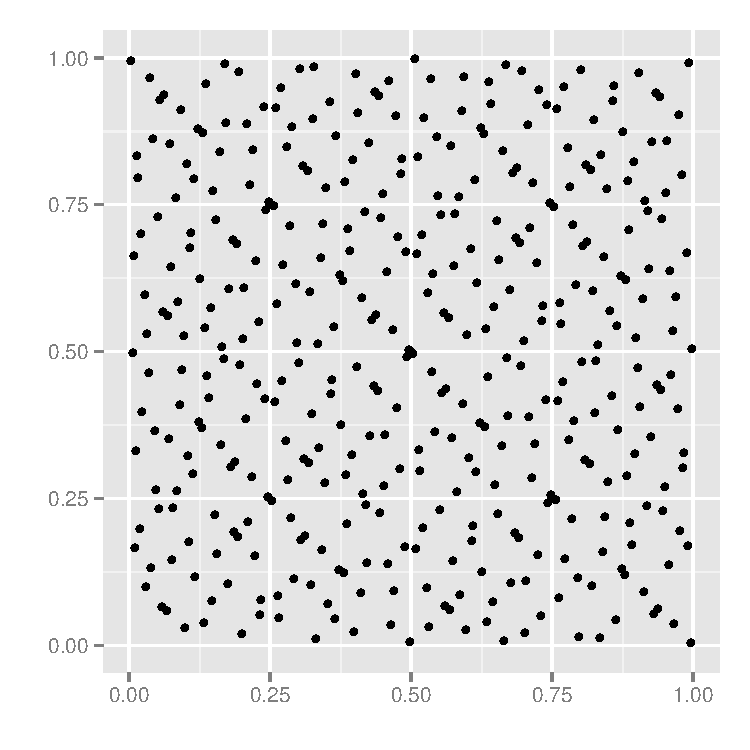
\includegraphics[width=0.45\textwidth]{graphics/2D-sobol-sequence.pdf}\hspace{0.55cm}\label{fig:2d-sobol-sequence}}
	\subbottom[]{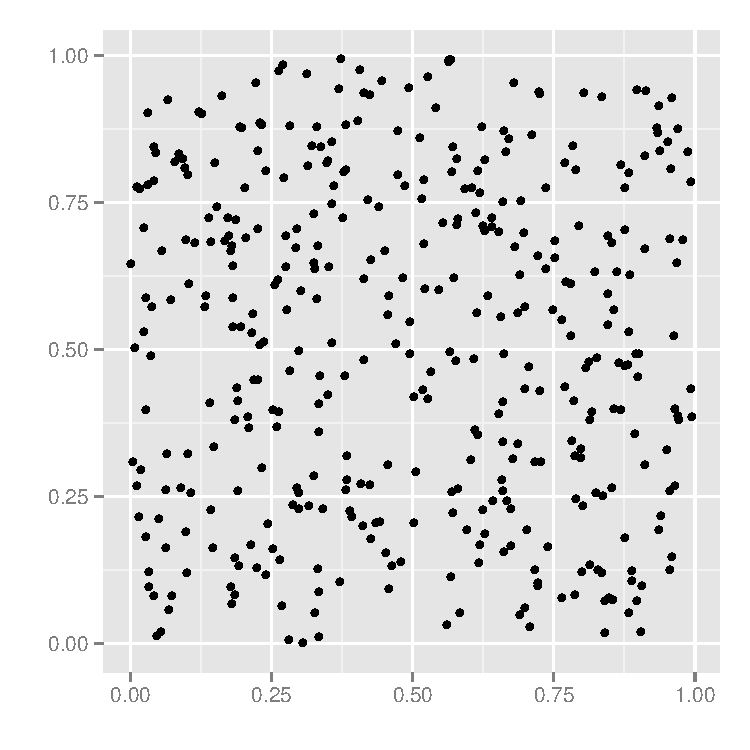
\includegraphics[width=0.45\textwidth]{graphics/2D-mersenne-sequence.pdf}\hspace{0.55cm}}

  \caption{\textbf{(a)} A 2D sequence of low-discrepancy numbers
    generated using the Sobol generator \textbf{(b)} A uniform 2D
    sequence of pseudorandom numbers generated with Mersenne twister
    PRNG}
\label{fig:discrepancyplot}
\end{figure}

QRNGs does not assure any other properties of random sequences and
does indeed follow rather visible patterns (see Figure
\ref{fig:2d-sobol-sequence}). It is not the aim to get close to
statistically random numbers, instead QRNG provides numbers suitable
for numerical integration, optimization and simulation. QRNGs have
several times been shown useful in financial Monte Carlo simulations
\cite{chaudhary2005american, couffignals2010quasi, dfine2009americanbasket}
%  \todo{perhaps mention the differences between their methods}
and a survey paper shows QRNGs beating PRNGs
when it comes to option pricing \cite{acworth1998comparison}. The
survey is 15 years old, so newer PRNGs might perform differently.
% \todo[noinline]{which other noteworthy?}

We will look closer at one particular low-discrepancy generator,
namely the Sobol sequence generator, by the Russian mathematician
I. M. Sobol \cite{sobol1967}. We chose the Sobol sequence because it
was the one used by an unrelated sample application from one of
HIPERFIT's industri partners. Also, the above mentioned survey
concludes that ``Sobol' points appear to give the best results among
the QMC sequences tested''.

\subsection{Sobol generator}
\label{sec:sobol}
We will not discuss why the numbers generated by the Sobol generator
maintain low discrepancy, but only focus on the algorithmic aspect of
computing the numbers.

Given a sequence of so called \emph{direction numbers}, $v_1, v_2,
\ldots$, the computation of Sobol-sequences is pretty straight forward:
$$x_i = b_1v_1 \oplus b_2v_2 \oplus \ldots \oplus b_lv_l$$
where $\ldots b_l\ldots b_3b_2b_1$ is the binary representation of $i$
in $l$-bit representation. This simple algorithm is presented in
Figure \ref{alg:sobol-inductive}, where \textsc{ToBitVector} converts
an integer $i$ to its binary representation as an array of
integers. We do not mentioned the used representation used, which is
also a factor of the implementation. In our own implementations we
have used $32$-bit integers. As computing each number is independent
of the other numbers, we can parallelise by mapping
\textsc{SobolInductive} over the indices.

The \textsc{SobolInductive} algorithm as well as the remaining
algorithms produces integer values in the range $[0, 2^l]$ and we thus
has to normalize this to $(0,1]$ to get a uniform distribution. In
addition, we have to convert this uniform distribution to a normal
distribution. This will be discussed in Section
\ref{sec:sampling_normaldist}.

\begin{algorithm}
  \begin{algorithmic}
    \Function{SobolInductive}{$v$,$i$}
    \State \Return \textbf{fold} $\oplus$ 0 (\textbf{zipWith} ($\times$) $v$ (\textsc{ToBitVector} $i$))
    \EndFunction
  \end{algorithmic}
  \caption{Generate element $i$ of the Sobol sequence using vector
    $v$ as direction numbers.}
  \label{alg:sobol-inductive}
\end{algorithm}

% \begin{algorithm}
%   \begin{algorithmic}
%     \Function{SobolInductive}{$v$,$n$}
%     \ParFor{$i \gets 0$ to $n-1$}
%     \State $A[i] \gets$ \textbf{fold} $\oplus$ 0 (\textbf{zipWith} ($\times$) (\textsc{ToBitVector} i) $v$)
%     \EndParFor
%     \EndFunction
%   \end{algorithmic}
%   \caption{Inductive Sobol generator.}
%   \label{alg:sobol-inductive}
% \end{algorithm}

If one seeks for a sequential algorithm for Sobol sequence generation,
we can improve on the above by using the Gray code binary
representation of the index instead of the ordinary, whereby a
recursive definition of Sobol sequences can be made
\cite{bratley1988algorithm}. It has been shown that
\begin{equation}
x_{n+1} = x_n \oplus v_c\label{eq:sobol-recurse}
\end{equation}

where $c = \mathit{lsb}(n)$ is the index of the least set bit in
$n$. A sequential algorithm using this strategy is presented in Figure
\ref{alg:sobol-recursive}.

\begin{algorithm}
  \begin{algorithmic}
    \Function{SobolRecursive}{$v$,$A$,$i$,$n$}
    \State $A[i] \gets$ \textsc{SobolInductive} (\textsc{GrayCode} $i$)
    \State $j \gets i + 1$
    \While{$j < i + n$ \textbf{and} $j < length[A]$}
    \State $c \gets \mathrm{lsb}(j)$
    \State $A[j] \gets A[j-1] \oplus v_c$
    \State $j \gets j + 1$
    \EndWhile
    \EndFunction
  \end{algorithmic}
  \caption{Generate elements $i$ through $i+n-1$ of the Sobol
    sequence and store results at the appropriate indices of $A$}
  \label{alg:sobol-recursive}
\end{algorithm}

This approach does not output the same sequence though, but it has
been shown \cite{bratley1988algorithm} that Gray code based sequences
also displays the property of low discrepancy, as it is merely a
scrambling (reordering) of prefixes of the original Sobol
sequence. Conversion to Gray code representation can be done through
single shift and an exclusive-or operation, which makes for a cheap
sequential algorithm.

The two approaches can be combined to achieve an alternative parallel
implementation. The sequence that needs to be generated is divided in
chunks onto each processing element, the inductive algorithm is used
to initialize each of the chunks and the recursive algorithm is then
used to fill out the space. The algorithm is shown in Figure
\ref{alg:sobol-parallel-1}

\begin{algorithm}
  \begin{algorithmic}
    \Function{SobolParRecurse}{$v$,$n$}
    \State $m \gets$ number of processor cores (e.g. CUDA cores)
    \State $r \gets \lfloor n/m \rfloor$
    \ParFor{$p \gets 0$ to $m-1$}
    \State $start \gets p\cdot r$
    \State \textsc{SobolRecursive}($v$,$A$,$start$,$\min(r,n-start)$)
    \EndParFor
    \EndFunction
  \end{algorithmic}
  \caption{Parallel Sobol sequence generator.}
  \label{alg:sobol-parallel-1}
\end{algorithm}

The problem with this algorithm is that its memory behavior is not
suitable for GPUs. Programs that does not coalesce memory accesses,
such that all cores act on the same block simultaneously, incurs a big
performance penalty. With this algorithm, each thread will write very
dispersed, as each thread will fill out each its own region of the
array A.

Luckily, an alternative strategy has been shown by Thomas Bradley et
al. \cite[Chapter~16]{hwy2011emerald}. They observed that applying
\eqref{eq:sobol-recurse} several times, would lead to repeated
exclusive or operations with the same direction number. As the
\emph{exclusive or} operation is associative, commutative and is its
own inverse, some of these operations will cancel out. Especially,
when skipping a power of two ahead, all but two exclusive or
operations will cancel out. The least set bit will change in a
systematic way, and analysis shows that (see the above mentioned book
chapter):

\begin{equation}
  \label{eq:sobol-skipahead}
  x_{n+2^p} = x_n \oplus v_p \oplus v_{q(n)}
\end{equation}

where $q(n) = lsb(n \blor (2^p - 1))$. We use $\blor$ for bitwise or.

This fact can be used to develop a parallel algorithm which is memory
efficient on GPU architectures. Instead of each letting each thread
fill a separate block of memory using \eqref{eq:sobol-recurse}, we can
instead let all threads cooperate on filling one block at a time, by
using the inductive algorithm (Algorithm \ref{alg:sobol-inductive}) to
fill the first block and use \eqref{eq:sobol-skipahead} to fill each
successive block. This thus requires a block size of a power of two.
\todo[noinline]{Can we do something smart if the block is not a power
  of two? Alternatively the section below should be changed, to say
  that we don't need information about block size, but need to
  actively control the block size.}

This also illustrates that optimized GPU algorithms in some cases
needs information about how kernel scheduling is performed, as we need
to know the size of a block to determine how much we have to skip
($p$).\todo{The survey should be aware of this: How much control do we
  have over kernel execution in Nikola and Accelerate? Is it possible
  to drop down to a lower layer for such implementations?}


% \begin{align}
%   x_{n+4} & = x_n \oplus v_{lsb(n)} \oplus v_{lsb(n+1)} \oplus v_{lsb(n+2)} \oplus v_{lsb(n+3)} \\
%          & = x_n \oplus v_1 \oplus v_1 \oplus v_2 \oplus v_3 \\
%          & = x_n \oplus v_2 \oplus v_3 \\
% \end{align}

\begin{algorithm}
  \begin{algorithmic}
    \Function{SobolSkipping}{$v$, $N$, $p$}
%    \State $p \gets$ number of processor cores (e.g. CUDA cores)
%    \State $r \gets \lfloor n/m \rfloor$
    \ParFor{$n \gets 0$ \textbf{to} $p-1$}
    \State $A[n] \gets$ \textsc{SobolInductive} (\textsc{GrayCode} $n$)
    \While{$n < N$}
    \State $q \gets lsb(n \blor (2^p - 1))$
    \State $A[n+2^p] \gets A[n] \oplus v_p~\oplus v_q$
    \State $n <- n+2^p$
    \EndWhile
    \EndParFor
    \EndFunction
  \end{algorithmic}
  \caption{Parallel Sobol sequence generator. $v$ is the direction
    vector, $N$ is the length of the sequence and $2^p$ is the block.}
  \label{alg:sobol-parallel-2}
\end{algorithm}

In the same book chapter they present skip-ahead strategies for two
PRNGs, the Mersenne Twister (the MT19937 variant) and L'Ecuyer's
Multiple Recursive Generator (MRG32k3a). \todo{Write some more about
  how they parallelise}

\subsection{Sampling the standard normal distribution}
\label{sec:sampling_normaldist}
The Sobol sequence generator as well as most other PRNGs and QRNGs
draws samples uniformly from the interval $(0,1]$ ($0$ is not
included, as we often want to avoid negative samples). In our
application we need samples from the standard normal distribution,
$\mathcal{N}(0,1)$, and thus a transformation is necessary.

The standard approach to convert from a uniform distribution to any
other distribution is by inversion of the cumulative distribution
function (CDF). It not possible to compute the inverted CDF exactly
for the normal distribution, but approximations exists. The algorithm
that seems the most popular when we have to do with QRNGs is called
the ``Beasley-Springer-Moro'' algorithm or ``Moro's inversion''. This
algorithm uses a result by Beasley and Springer from
\cite{beasley1977algorithm} to approximates the inverse CDF of the
standard normal distribution by
$$norminv_1(u) = \frac{\sum^3_{n=0}a_n(u-1/2)^{2n+1}}{1+\sum^3_{n=0}b_n(u-1/2)^{2n}}$$
on the interval $u \in [0.5, 0.92]$ for a specific set of constants
$a_n$ and $b_n$, see \cite[page 67-68]{glasserman2003monte}. Boris
Moro found \cite{moro1995full} that he could approximate the remaining
interval $u \in (0.92, 1]$ by $$norminv_2(u)= \sum^8_{n=0}c_n
log^n(-log(1-u))$$ where $c_n$ are additional constants, also given in
\cite{glasserman2003monte}. With this, the inverse CDF of the standard
normal distribution can now be written as:
$$cdf^{-1}(u) = \left\{
\begin{array}{ll}
  norminv_1(u) & \mathrm{if}~ 0.5 \leq u \leq 0.92\\
  norminv_2(u) & \mathrm{if}~ 0.92 < u < 1\\
  - cdf^{-1}(1-u) & \mathrm{if}~0 < u < 0.5\\
\end{array}\right.$$

\subsection{Least Squares solvers}
The only remaining element of the Longstaff \& Schwartz algorithm that
we need to discuss is the least squares regression. What we need is a
way of smoothing out the variation in the paths, by representing their
change from one point in time to the next by a function. We have a set
of stock prices $S_t$ and a set of option values $V_t$ and wants to
find the polynomial $f$ of a degree $d$ that is as close to these
coordinates as possible. That is, we want the coefficients
$\mathbf{x}$ for the polynomial that minimizes the error:

$$min_\mathbf{x} \sum^{N}_{i=0}(V_{t,i}-f(S_{t,i},\mathbf{x}))^2$$

to generalize this, we will use $a$ and $b$ in the rest of this
section, such that:
$$min_\mathbf{x} \sum^{N}_{i=0}(b_i-f(a_i,\mathbf{x}))^2$$

In our case, $f$ will take the shape of a polynomial:
$$f(\mathbf{a},\mathbf{x}) = x_1 + x_2a_i + x_3a_i^2 \ldots x_da_i^{d-1}$$
and this gives rise to a linear system of equations. Each equation
originating from a coordinate $(a_i, b_i)$. We write the system as:

\begin{equation}
  \label{eq:vandermonde}
  \mathbf{Ax} =
  \left(
  \begin{array}{ccccc}
    1 & a_1 & a_1^2 & \ldots & a_1^{d-1} \\
    1 & a_2 & a_2^2 & \ldots & a_2^{d-1} \\
     & & \vdots & & \\
    1 & a_n & a_n^2 & \ldots & a_n^{d-1} \\
  \end{array}\right)
  \left(
  \begin{array}{c}
     x_1 \\
     x_2 \\
    \vdots \\
     x_n \\
  \end{array}\right)
=
  \left(
  \begin{array}{c}
     b_1 \\
     b_2 \\
    \vdots \\
     b_n \\
  \end{array}\right)
= \mathbf{b}
\end{equation}

The $\mathbf{A}$ matrix is called a Vandermonde matrix.  To find the
minimizing $x$ vector, we want to minimize the residual vector
$\mathbf{r} = \mathbf{b} - \mathbf{Ax}$. By \todo{magic} we know that
we can find the minimizing $\mathbf{x}$ by solving the system
$\mathbf{A}^T\mathbf{A}\mathbf{x} = \mathbf{A}^T\mathbf{b}$.

There are several ways to solve such systems, for instance
LU-decomposition, QR-decomposition or Cholesky-decomposition. We have
chosen to implement Cholesky-decomposition, though that choice was a
bit arbitrary.

With Cholesky decomposition we find a lower triangular matrix
$\mathbf{L}$ such that $\mathbf{A} = \mathbf{LL}^T$. And now forward
and then backward substitution can be used to find the minimizing
$\mathbf{x}$.

%%% Local Variables:
%%% mode: latex
%%% TeX-master: "../master"
%%% End:



%%% Local Variables:
%%% mode: latex
%%% TeX-master: "master"
%%% End:


\part{Survey}
\part{Survey}
\chapter{Survey Setup}
In this and the following chapters we present a small-scale survey of
current vector languages. The survey was originally conducted to
orient ourselves in the current landscape of parallel functional
languages and their implementation, but the results might be of
interest for others. We do not know of other comparisons with similar
scope.

\section{Languages}
We have decided to evaluate and compare the languages Accelerate
\cite{chakravarty2011accelerating}, Repa \cite{keller2010regular},
Nikola \cite{mainland2010nikola} and the \texttt{Data.Vector}
package\footnote{\url{http://hackage.haskell.org/package/vector}}. We
compare these four libraries to the R programming language and NVIDIA's
CUDA platform, which are some of the languages currently used by
financial engineers. The R language is used for expressing financial
algorithms succinctly, while CUDA is used for performance reasons,
which is why we have chosen to include both of these. Because of time
constraints, we have had to limit ourselves more than we had originally
intended. This means we have had to leave out languages such as
Feldspar\cite{axelsson2010feldspar},
Obsidian\cite{svensson2011obsidian}, Data Parallel Haskell \cite{},
Copperhead\cite{Catanzaro2011} and NESL\cite{nesl} from the survey,
although they might have provided further insights.

\todo{Why only Haskell? Are there any languages we have left out
  entirely? What about Theano, ArBB, Qilin, Erlang, SaC, CnC-CUDA? Why
  aren't they here?}


We will now look a bit closer on each of the chosen languages. If you
already have experience in this area, you can skip this section.

\subsection{Data.Vector}

\subsection{Repa}

\subsection{Accelerate}

\subsection{Nikola}

\section{Programming language surveys}
To make a fair comparison, we have to be objective in our evaluation
of the languages. Obtaining objectivity in such a comparison is not
an easy task, as it is hard to quantitatively measure aspects such as
the quality of language documentation (longer is not always better,
and it might be outdated). Also, as mentioned by Lutz Prechelt in his
2001 paper ``Empirical Comparison of Seven Programming Languages'':

\begin{quote}
  ``Any programming language comparison based on actual sample programs
  is valid only to the degree to which the capabilities of the
  respective programmers using these languages are similar.''
\end{quote}

We would thus have to either acquire the same level of experience in all the
languages ourselves or find experts in each of the languages to do the
implementation. We have not had the resources to conduct a survey
following the standards set in the paper by Lutz Prechelt. For each
language under comparison he acquired 10-20 implementations of the
same algorithm from different programmers (mostly graduate
students). We could have set up a similar experiment by presenting a
programming challenge to the ``Haskell-Cafe''-mailing list and/or the
Haskell section on the Reddit website, and surely we could perhaps get
a decent benchmark in terms speed and memory usage for different
implementations by different developers, but we would not get answers
to qualitative questions about the development process. Another aspect
is that these languages are all in their early stages, and most people
we would find on those channels might be amateurs. We do not find
amateur work a good basis for an objective comparison.

\todo{could still be an interesting experiment to make in the future.}
\todo{look through the above argument again}

\section{Comparison}
From the survey we want to uncover three main questions about each
language, and it is from answers to these questions that we will make
a comparison. The three questions revolve around the health of
project, the expressiveness and ease of use of the language, and the
performance of the language. The following three sections will pose
these questions and describe how we have decided to test them.

\todo{Should we also include an evaluation on ``Performance
  \textit{guarantees}''? That is, an evaluation of the theoretical
  aspects and cost models?}

\subsection{Project Health}
How good is the project health? That is,
we want to determine how likely is it that development on the language
will continue and that it will keep getting funding and interest from
developers.

Subquestions include:
\begin{itemize}
\item Quality of documentation. Good documentation gives better acessibility for new users and developers.
\item Code review. Our own assesment of the standard of the code.
\item Portability. More portable progams have a wider potential user audience.
\item Installation process. A cumbersome installation process is deterring for newcomers.
\item Number of dependencies (incl. GHC extensions). ``Bad health is transitive''.
\item Number of users (reverse dependencies). The bigger the audience, the more people with some interest in the project continuing.
\item Number of contributors.
\item How easy is it to start contributing?
\item Latest project activity (e.g. which version of GHC does it compile on?)
\item Licensing
\item Funding
\end{itemize}

\todo{Document the procedures and scripts that were used to collect reverse dependencies and to carry out installs}

\subsection{Ease of use and expressiveness}

How easy is the language to use? And how expressive is it? Our
aim is to find a language that might be suitable for a financial
engineer and we thus want a suitably high-level language. It should
be near the complexity level of R. We still want the language to
expressive enough to cover the domain of financial algorithms.

Subquestions include
\begin{itemize}
\item Which programs can we write, and which can't we write?
  \begin{itemize}
  \item Can we write nested loops?
  \item Does it include all of: scans, folds, zip/map, stencils,
  \end{itemize}
\item How good are the error messages?
\item How high-level is it on the scale from ``R'' to ``CUDA''?
\end{itemize}

\subsection{Performance} How does the languages compare in a
performance benchmark?
\begin{itemize}
\item Benchmark of binomial pricer on expiry = 1,2,4,8,16,32,64,128 years.
\item Benchmark of Longstaff and Schwartz
\item Which optimizations are performed?
\item How many in-code optimiser hints (inlining-statements, forcing
  of delayed arrays etc.) are necessary to get decent performance?
\item How does the performance of a naive implementation (no
  optimiser hints) compare to an optimised version?
\end{itemize}


%\begin{itemize}
%\item How do we carry out the survey?
%\item How are such surveys normally performed?
%\item Which parameters do look for and measure?
%\item How do we measure these things, e.g. how do we evaluate ``project health''?
%\item Why didn't we include some languages, but included others?
%\end{itemize}

\chapter{Evaluation: Project Health}
%``How good is the documentation?'',

\section{Accelerate}
\subsection{Source Quality}

\paragraph{Documentation.} The documentation for Accelerate resides mainly in
two different places: The haddock API-docs on hackage, and more high-level
documentation on the project's github wiki.  Other documentation reside in
somewhat scattered web pages, most notably in the paper
\cite{chakravarty2011accelerating}.  As of this writing, the main introductory
material seems to be the github project wiki and the paper
\cite{chakravarty2011accelerating}. Of these two, the wiki pages are more
oriented towards building applications using Accelerate, while the paper
focuses on detailing the current implementation and only briefly introduces the
Accelerate language in an academic fashion.

Unfortunately, many of the wiki pages are rather incomplete, so we must
conclude that there has yet to be published any comprehensive introductory
material on programming using Accelerate.
The API reference documentation however is extensive.

\paragraph{Code.} The Accelerate codebase is large for a Haskell library, and
a bit overwhelming at first. They have a good division between frontend (the
accelerate package) and backends (e.g. the accelerate-cuda package), which
limits the amount of code you have to get into. You don't really have to
understand the complete frontend to modify in the backend and vice versa. A
good overview document of the different modules, and their tasks would be a
great benefit for getting other hackers involved.\todo{Text above is copied
verbatim from wiki.}

\paragraph{Installation process} We succeeded in getting Accelerate to run on
GHC 7.4.2, but it still doesn't support GHC 7.6.1, possibly because of external
dependencies.  We had some trouble installing the version on hackage, because
of a minor bug in the cuda-bindings. The bug was caused by code generated by
c2hs, so it might be something that depends on the version of CUDA installed.

We had major trouble installing the development-version from their repository,
mainly caused by a lot of dependency issues and conflicts. We still have to
compile the CUDA-backend.  \todo{Text above is copied verbatim from wiki.}

\subsection{Relations with other projects}

\paragraph{Dependencies.}
For the Accelerate frontend we have counted 8 package dependencies and 19 GHC
extensions, while the CUDA backend sports 23 package dependencies and 5 GHC
extensions.
Most of the package dependencies are commonly occuring packages, but some are
less so. \todo{The last paragraph sounds unsubstantiated}

The Accelerate frontend is tied only to the GHC-compiler (through its generous
use of GHC haskell extensions), and thus runs on any platform (architecture or
OS) that GHC supports.
The CUDA backend is only available on machines with a NVidia CUDA graphics
card, and supports all versions of CUDA (but recommend using at hardware with
at least compute capability 1.2).

\paragraph{Reverse Dependencies.} For Accelerate we have
counted a total of two package users on hackage, excluding the different
accelerate backends, as we consider them to be part of the same project.

\paragraph{Contributors.} During the last 12 months, the Accelerate
frontend has seen a total of 6 different contributors. Across the entire
project history, 14 people have contributed.
Accelerate is hosted as a git repository on github.com, so getting a copy of
the latest source code and submitting patches is structurally
straightforward.
Given that the project has seen a variety of small volume contributers, with no
apparent close connection to the Accelerate maintainers, they appear to have an
inclusive attitude towards other people's code.

\paragraph{Licensing.} Accelerate is licensed under BSD-like terms, requiring
mainly that attribution is retained in derivative works.

\subsection{Maintainance}

Accelerate has been actively maintained for the
past 12 months.
The two main contributors, Trevor L. McDonell and Manuel M
T Chakravarty, are both employed by University of New South Wales, Sydney,
Australia, and assumably maintain Accelerate as part of their research there.

\section{Repa}

\subsection{Source Quality}

\paragraph{Documentation.} Repa is extensively documented through both API
documentation on hackage, various papers, tutorials and example programs, eg in
\cite{lippmeier2012guiding} and \cite{keller2010regular}.  Everything is easily
accessible directly from the front page of the repa homepage
\cite{homepage:repa}.

\paragraph{Code.}
\todo{\ldots}

\paragraph{Installation process.} Since Repa is just a regular Haskell package
that doesn't interface with foreign functions, its installation is
straightforward using the \texttt{cabal-install} program.

\subsection{Relations with other projects}

\paragraph{Dependencies.} %
Repa uses 18 GHC extensions and depends on 6 other established packages, none
specific to any platform. Thus, Repa will most probably function on any
machine that is targetable by GHC.

\paragraph{Reverse Dependencies.} Repa is a comparatively popular package. On
hackage there are 9 other packages that each depend on Repa.

\paragraph{Contributors.} Looking at the commit log for the official Repa
source code repository, we may count 4 distinct names. The primary contributor
(in number of patches) appears to be Ben Lippmeier by a great margin.

\todo{It seems redundant to keep saying that the code is publically available
in a VCS. They all are. And we have no reference to cite that contributions are
welcome, so any comment on contribution friendliness would be guesswork. Should
we perhaps report that? Is the question of ease of contribution even
interesting? Isn't it a universally accepted work dynamic of free/oss software
that contribution is encouraged}

\paragraph{Licensing.} Repa is licensed under the terms of the BSD3 license.

\subsection{Maintainance}
Ben Lippmeier is employed as a researcher by "School of Computer Science and
Engineering", and Repa is listed among his projects there.

\section{Nikola}

\subsection{Source Quality}

\paragraph{Documentation.} As Nikola is not published on Hackage, there is no
automatically searchable generated documentation, and one has to manually
generate haddock documentation. Counting source lines reveals a figure of 24\%
comment lines, which is above the average comment ratio according to the
ohloh.net open source project visualisation website\footnote{14-11-2012:
``Across all Haskell projects on Ohloh, 17\% of all source code lines are
comments. For nikola-haskell, this figure is 24\%.''} Further, Nikola is
described in the paper \cite{mainland10nikola}.

\paragraph{Code.} (TODO)

\paragraph{Portability.} Only runs(/builds even?) on machines with an NVidia
CUDA card and with the CUDA drivers and sdk installed.

\paragraph{Installation process} Nikola requires running a classical style
automake "configure"-script to produce the binding to the cuda-backend.

We had a sizable amount of trouble executing the installation. \todo{why
exactly? (Difficult to link with CUDA sdk, cabal dependency hell)}

\subsection{Relations with other projects}

\paragraph{Dependencies.} For Nikola we have counted a total of 20 package
dependencies, all of which are either maintained by Mainland himself or appear
to have a healthy user base (reverse dependencies on Hackage).

One of the dependencies is the \texttt{cuda} package, meaning that the nikola
package is only installable on machines with the NVidia CUDA sdk and hardware.

We have counted the use of 26 different GHC language extensions, most of which
are regularly occuring. \todo{We need a more purposeful/relevant treatment of
ghc extensions and their consequences to project health}

\paragraph{Reverse Dependencies.} Since Nikola is not published on hackage, our
method of counting users doesn't apply. Nikola is published on the github.com
website however, where the project has 9 stars and zero forks\footnote{Gathered
on 2012-11-15}, which is at least some measurable artifact of the existance of
human interest in the language effort.

\paragraph{Contributors.} According to the version control system's commit
logs, only Geoffrey Mainland has contributed to the development of Nikola

The source code is hosted on github, so structurally/bureaucratically easy.
Geoffrey appears to be interested/open in merging in contributions from other
people. \todo{This comment still seems redundant ..}

Since Nikola is still a work in progress that has yet to settle on a final form
and direction, new contributions might only be accepted if they align with the
author's own possibly unarticulated notion of what he wants with the project.
\todo{This needs reassesment..}

\paragraph{Licensing.}
Harvard College, appears BSD style. \todo{validate or elaborate.}

\subsection{Maintainance}
\todo{ Appears to have been funded as part of phd research (or what?), but appears
to be a spare-time project now.}

\section{Data.Vector}

\subsection{Source Quality}
\paragraph{Documentation.}
\paragraph{Code.}
\paragraph{Portability.}
\paragraph{Installation process}

\subsection{Relations with other projects}
\paragraph{Dependencies.}
\paragraph{Reverse Dependencies.}
\paragraph{Contributors.}
\paragraph{Licensing.}
\subsection{Maintainance}


\begin{table}
  \centering
  \begin{tabular}{l|rrllllr}
    Language    & Project age & Latest release & License & Contributors \\ \hline
    Accelerate  & 3-4 years   & June 2012      & BSD3    & 3 \\
    Nikola      & 1-2 years   & Not released   & BSD3    & 1 \\
    Repa        & 1-2 years   & October 2012   & BSD3    & 4 \\
    Data.Vector & 4 years     & October 2012   & BSD3    & 9 \\
  \end{tabular}
  \caption{Project status}
  \label{tab:project_status}
\end{table}

\begin{table}
  \centering
  \begin{tabular}{l|rrllllr}
    Language    & Dependencies & Reverse dependencies & GHC extensions & GHC version \\ \hline
    Accelerate  & 5 (+18)      & 2                    & 19 (+9)        & 7.6.1 \\
    Nikola      & 21 0         & 0                    & 26             & 7.4.2 \\
    Repa        & 6            & 11                   & 20             & 7.6.1 \\
    Data.Vector & 4            & 150+                 & 15             & 7.6.1 \\
  \end{tabular}
  \caption{Dependency status}
  \label{tab:dependency_status}
\end{table}


\chapter{Evaluation: Expressiveness}
% ``How tight is the correspondence to the Rolfs R-code?''

\chapter{Performance}
We will now look at how the different languages compare in performance
and which optimisations they employ.

\section{Optimisations}

\subsection{Data.Vector}
The documentation on Data.Vector is scarce, what we know is that it
performs some fusion, and a single comment reveals that they use the
foldr/build deforestation algorithm introduced in ().

\subsection{Accelerate}
Fusion is currently being implemented in Accelerate. The newest
version on Hackage (0.12.1.0) does not perform any fusion, but the
development repository contains a not completely functional
implementation, so it will possibly be part of the next release.

Accelerate goes a long way to restrict the possible programs you can
write, such that they can make certain performance guarantees. For
instance, they do not allow you to write sequential loops running on
the GPU as this may allow one thread to diverge letting the remaining
threads in a block waiting.

This is problematic, as certain problems are more efficiently
expressed using nested loops, and you thus need to manually flatten,
giving a performance penalty. Techniques have been developed to
minimise thread divergence, and as such they could possibly benefit
from such an implementation.


\section{Benchmarks}
Speed up graph. In the graph we use the sequential version written
with Data.Vector as our basis, which the others are compared to.

Accelerate is not included, because of problems in their stream fusion
algorithm leading to running times that evolve
exponentially. Disabling fusion lead to CUDA exceptions.

We see that the overhead incurred by using Nikola makes both
sequential implementations (R and Data.Vector) faster for the smallest
cases, and only when we reach the largest example (128 years expiry
time) Nikola catches up.

Repa is the best performing, even though it does not perform any GPU
computations. We are not sure why Repa gives so varied speed-ups for
different input sizes, but it might be because of our somewhat
arbitrary threshold for which problem sizes should be executed in
parallel and which should be executed sequentially.


\chapter{Conclusion}
What are our recommended choice of languages for different use-cases?

%%% Local Variables:
%%% mode: latex
%%% TeX-master: "master"
%%% End:



\part{Language Extension}
\chapter{Nikola} % or 'Nikola elaborated' or similar.

\todo{Introduce nikola. The choice of nikola should already have been documented in the conclusion of the survey}
 % maybe nikola/description.tex is sufficient.
\section{Frontend Architecture}

In this section we describe the part of Nikola that serves as the language
programming interface, as well as the middle layer which is still backend
agnostic.

The Nikola language is made up of three data types: \texttt{Exp t a},
\texttt{Array r sh a} and the program monad \texttt{P a}. These parts are all
backend agnostic. It also provides a type class directed \texttt{compile}
function for compiling Nikola functions to CUDA code which is subsequently
wrapped as regular haskell functions. \texttt{Exp t a} expressions are first
translated to another first-order untyped abstract syntax before CUDA code
generation.

\paragraph{Nikola scalar expressions} are represented by the \texttt{Exp t a} type, with
the phantom type variable \texttt{t} representing the target architecture for
the expression, eg.  \texttt{CUDA}. Thus, it is possible to have Nikola terms
specialised for different backends. This is unusual, as programming languages
are typically assumed universal in the sense that every well-typed expression
is executable on every supported machine architecture. Nikola is the first
programming language we have witnessed to explicitly encode term portability in
the type system. However, the ability to specialise expressions to targets
doesn't extend into the lower layers of Nikola, so as such the \texttt{t} type
variable only clutters up type signatures currently.

\paragraph{Arrays in Nikola} are modeled by the type \texttt{Array r sh a}, an associated
type of the typeclass \texttt{IsArray r a}. Arrays are parametrised on their
representation and shape by the type variables \texttt{r} and \texttt{sh},
following in the tradition of Repa. The only common operation for all arrays is
that of extracting their shape through the function \texttt{extent}. Array
shapes are similar to those of Repa and Accelerate, denoted as instances of
typeclass \texttt{Shape sh}.

Three principal array representations are provided by Nikola: The global array,
the delayed array, and the push array, denoted respectably by the types
\texttt{G}, \texttt{PSH} and \texttt{D}. This is a source of both control and
complexity, as each representation gives rise to different features and
restrictions. The global array represents a certain manifest range of memory
cells, from which it is only referentially safe to read. Push arrays and
delayed arrays however, represent array computations rather than actual areas
of memory - only at the Nikola-Haskell border are they manifest into memory. An
important consequence of this is that terms composed of delayed and push arrays
undergo fusion by construction.

What distinguishs push arrays and delayed arrays is their perspective on the
arrays they represent. A delayed array is simply a function from indices to
values, while a push array may be viewed as a stream of index/value pairs, that
may appear in potentially any ordering.

\paragraph{The type of the low-level abstract syntax} is \texttt{S.Exp},
qualified to avoid confusion with \texttt{Exp t a}. This is elaborated in the
nikola reference in section \ref{section:nikola-reference}.  \texttt{S.Exp}
defines primitive constructs for annonymous functions, delayed arrays,
accessing and manipulation of mutable arrays, and a \texttt{for}-loop
construct. Many of these constructs map directly to corresponding C constructs.

\paragraph{The monad \texttt{P a}} serves some of the same roles as the
\texttt{IO} monad does in plain Haskell. One must for example only manipulate
mutable arrays from within the \texttt{P} monad.  It is a type alias for the
slightly more elaborate monad type \texttt{type P a = R S.Exp a}. The monad
\texttt{R r a} is the reification monad, used to convert the various
frontend datatypes such as \texttt{Exp t a} and \texttt{Array r sh a} into the
low-level abstract syntax \texttt{S.Exp}.

To enable this, monad \texttt{R r a} is a continuation monad.  \todo{for
now just assume knowledge of continuation passing monads :-(} But instead of
direct access to the underlying continuation, Nikola uses delimited
continuations, described in \cite{wadler1994monads} and introduced first in
\cite{filinski1996controlling}.
The interface to using delimited continuations consists of two special operations:

\begin{verbatim}
shift :: ((a -> R r r) -> R r r) -> R r a
reset :: R r a -> R r r
\end{verbatim}

Which when specialised to the \texttt{P} monad becomes:

\begin{verbatim}
shift :: ((a -> P S.Exp) -> P S.Exp) -> P a
reset :: P a -> P S.Exp
\end{verbatim}

\texttt{shift} and \texttt{reset} work in tandem. A full account of the use and
details of delimited continuations is out of scope for this thesis, but
consider this short typical usage pattern:

\begin{verbatim}
reset $ do
  ...
  y <- shift $ \k -> do
    ...
    x <- k ""
    ...
  ...

\end{verbatim}

In this \texttt{shift} expression, \texttt{k} is a continuation representing
all that is going to happen up until the enclosing \texttt{reset}.  Upon
invoking \texttt{k ""}, control shifts outside of \texttt{shift}, and \texttt{y}
is bound to the empty string \texttt{""}. Upon reaching the end of the monadic
action inside \texttt{reset}, control is shifted back into \texttt{shift}, and
\texttt{x} is bound to the result of the enclosing action. The eventual result
of the action inside \texttt{shift} then becomes the result of the enclosing
\texttt{reset}. Informally, \texttt{shift} and \texttt{reset} turn the code
inside-out.

\section{Nikola Backend Architecture}

In this section we describe some parts of Nikola that are used for code
generation.

Compiling a Nikola function relies on both reification to \texttt{S.Exp}, a
mechanism to determine the type of the resulting haskell function, and the
translation from \texttt{S.Exp} abstract syntax to C abstract syntax.

Reification is handled by the function \texttt{reify :: Reifiable a b => a -> R
b b} of typeclass \texttt{Reifiable}.

The programmer is \ldots \todo{explain how Compilable a b instance selection allows for different resulting haskell wrapper types}
  % describe the architecture of nikola. Identify extension points.
\chapter{Extensions}
\chapter{Iterative array construction}
\label{chap:unfold}
% Disposition
% * Chapter overview
% * Define our need
% * Tell that there are two possible solutions
% * Present solution one: NDP approach
%   - Show where it breaks down, what are we missing
% * Present solution two: Accelerate approach
%   - Tell how it could be used in Accelerate to solve our problem
%   - That it would be possible to implement directly into the Accelerate architecture
% * Discuss the two approaches
%   - With one world view one is better, with another the other is better.
%   - Depends on the point of view

% (* Tell that we implemented a version in Repa
%   - It did what was necessary for us.
%   - We believe it is an addition that might be worthwhile,
%     as we think it is general enough to suit other problems
%   - Show graph of execution speed versus the best performing
%     solution we have without the new construct)

In this chapter we present our takes on adding support for expressing
iteratively defined arrays. Unfortunately we have not been able to get any of these
extensions completely ready for use and possible inclusion into Nikola.  We
will however give an analysis of what is lacking for a more complete
implementation.

Our need to iteratively define arrays is motivated directly from our
case work on the variants of the recursive Sobol-sequence generator
and the LSM path generator, depicted in Algorithms
\ref{alg:lsm-pathgeneration}, \ref{alg:sobol-recursive} and
\ref{alg:sobol-parallel-2}.  While in general the needs for a specific
example does not always warrant language extensions, the case of
incremental construction of output data is arguably a common one, and
thus well motivated.

But in isolation, the ability to construct a single array iteratively
is insufficient. It must also be possible to produce multiple
iteratively constructed arrays in parallel. This is due to both the
desire for performance and the desire for expressivity. To meet this
end we will analyse two possible ways to go about this: a version
using nested array operators and a flat parallel version.

\section{Nested array operators}

Since it is not possible to use recursion in Nikola, we must implement
a primitive iterative operator to incrementally construct arrays. In
Haskell, a function with a similar effect is \lstinline{unfoldr} of
the \lstinline{Data.List}-module:
\begin{lstlisting}
unfoldr :: (b -> Maybe (a,b)) -> b -> [a]
\end{lstlisting}
It recursively populates the element of a list with \lstinline{f}, as
long as it evaluates to a \lstinline{Just}-value. It is a well known
way to construct a list, which further motivates it as an addition to
Nikola.

In Nikola the length of an array is the only intrinsic property shared
across all array representations. Therefore we must know the length of
the result array a priori to evaluating a Nikola
\lstinline{unfoldr}. For a prototype that only uses the last generated
element as state, we settle for the type signature:
\begin{lstlisting}
unfold :: (Shape sh, IsElem a, Typeable a) 
       => sh -> (sh -> a -> a) -> a -> Array PSH sh a
\end{lstlisting}
In order to be useful however, \lstinline{unfoldr} by itself is not
enough. We need to be able to iteratively produce entire rows or
columns of a matrix as required in Algorithm
\ref{alg:lsm-algorithm}. To remedy this, we set out to explore nested
maps. Again, lacking nested arrays we must use array shapes to express
the structure of our computation.  Like in the case of
\lstinline{unfoldr} we thus must express the resulting shape
beforehand.

The type we eventually arrived at for our maps capable of nesting is depicted
here:
\begin{lstlisting}
mapNest :: (Shape sh, Shape sh', IsElem a, 
            IsElem (Exp t Ix), IsElem b, Source r a)
        => sh'
        -> (Exp t Ix -> Array D sh a -> Array PSH sh' b)
        -> Array r   (sh :. Exp t Ix) a
        -> Array PSH (sh' :. Exp t Ix) b
\end{lstlisting}

While we require the shape \lstinline{sh'} to be specified, there is no guarantee
in the application \lstinline{mapNest f xs} that \lstinline{f x} will not produce an
array exactly the size denoted by \lstinline{sh'}. If the resulting array is
smaller than denoted by \lstinline{sh'}, an eventual manifestation of the map to
memory will leave some cells uninitialized. Similarly, if the resulting array
is not bounded by \lstinline{sh'}, manifesting it will result in writing out of
bounds.

For now we have chosen to accept the existence of these fallacies,
partly because we are concerned with implementing a prototype, and
partly because we do not see any acceptable resolution of the problem
beyond placing the actual array extent rather than just the shape into
the type of the array, as done in \cite{thiemannagda}, but such a
change to Nikola is outside the scope of our project.

Another issue with this definition is the \lstinline{Source r a} restriction on
\lstinline{xs}. If the mapped function does not need to index into the array, it
is an unnecessary restriction to impose.  Similarly, if the mapped function
performs only elementwise operations, preserving the property of being
indexable would be valuable to retain for possible further processing of the
result array.

Risking to further complicate the types, the situation is somewhat remediable
by defining \lstinline{mapNest} as a function in a typeclass parametrised over the
involved array representations, as is already the case for typeclass
\lstinline{Map}.

The most important issue about this definition however, is that it permits
expressing nested array operations, which is not directly executable on the flat
parallel hardware. Treating this issue is the subject of Chapter
\ref{chap:directing-parallelism}.

\subsection{The inadequacies of our implementation}

All our efforts on iterative array construction draw on Nikola's implementation
of 'push' arrays. As mentioned earlier, delayed arrays and push arrays are each
others opposites. Delayed arrays are \lstinline{Source} arrays, and their
manifestation is at the mercy of the consumer of the array. Therefore it is
required that the elements of a delayed array are completely independent from
each other. Push arrays on the other hand are defined as a stream of
index-value pairs, and thus need not obey the same restriction on element
dependence.

Push arrays in Nikola are defined by means of the loop constructor
\lstinline{ForE} of \lstinline{S.Exp}. This loop constructor however, is very
low-level in the sense that it includes as arguments a list of variables to be
looped over and a list of loop bounds corresponding to each of the variables,
and corresponds directly to a \lstinline{for}-loop in C.

% The \lstinline{Shape} typeclass defines an accessible interface for constructing
% for-loops that visit each index of given shape to loop over.  The operation
% \lstinline{seqfor :: Shape sh => sh -> P sh} that we use for constructing our
% loops is defined using the \lstinline{shift} action, and thus needs to be paired
% with an enclosing \lstinline{reset}.  Due to the way that \lstinline{shift} operates,
% what happens is that upon issuing \lstinline{seqfor} in the \lstinline{P} monad, the
% entire surrounding action up to the nearest enclosing reset is placed inside
% the body of the for-loop defined by \lstinline{seqfor}.

However to our regret, using this approach for defining \lstinline{unfold} and
\lstinline{mapNest} proved unfruitful, as the part of the C code generation that
pertains to for-loops in Nikola does not handle cross-iteration data
dependencies properly. It assumes that variables that are overwritten inside
the body of the loop constitute new, fresh variables. Due to our time
constraints we were not able to address this, and have to leave our operations
be for now. If however we disregard this problem, we are not aware of any more
obstacles for implementing our extensions properly.

\section{Flat data parallel version}
Our first attempt at defining an unfolding operation was inspired by the
collective operators of Accelerate.

\begin{lstlisting}
unfold :: (IsElem a, IsElem (Exp t Ix), Shape sh, Source r a)
       => Exp t Ix
       -> (Exp t Ix -> a -> a)
       -> Array r sh a
       -> Array PSH (sh :. Exp t Ix) a
\end{lstlisting}

By avoiding the need for a nested array operations, it is guaranteed
that the resulting unfolded arrays are regular. Furthermore, since the
operation is a mapped version of \lstinline{unfold}, the outer
structure of the computation is completely static, and it is possible
to assign a parallel execution semantics, given that the unfolded
function is executed sequentially.

As such it fits quite well with the other array operations in Accelerate. If it
were to be implemented in Accelerate, it would enable us to express the
optimised version of Sobol sequences, Algorithm \ref{alg:sobol-parallel-2},
which is currently inexpressible.

\todo{explain}

\section{Discussion}
Which of the two possible implementations to select depends on ones
point of view. From one point of view, all programs that type checks
should be correct and come with guarantees of good performance. As we
have seen this style does in some cases break program composability,
but the other aspects are certainly also worth pursuing.

In this case, we find that the one invariant a developer has to
manually enforce when applying our \lstinline{mapNest} is worth the
extra cost in man hours, when compared to reading and writing programs
in the style we have seen in Section \todo{ref}.

%%% Local Variables:
%%% mode: latex
%%% TeX-master: "../master"
%%% End:
  % unfold and mapNest. Also displays gpu-gem sobol.
\chapter{Par/Seq evaluation}

\todo{Here we describe our extension idea of the 'sequential' operator, what it
would do to expressivity, and what it appears to enable for performance tuning
(i.e. deciding the degree of parallelism). Also, we describe how we implemented
it, or if we don't get to it, how it might be implemented.}
 % if time permits, describe (or code!) the parseq execution model and the 'sequential' operator.

% Make space in the table of contents so the conclusion and
% bibliography is separate from the Language Extension-part
\addtocontents{toc}{\protect\vspace{10pt}}

\chapter{Conclusion}
\label{chap:Conclusion}
\section{Future Work}


\subsection{Nested data-parallelism on NVIDIA Kepler GPUs}
On newer GPUs supporting CUDA 5.0, such as the one we have had access
to, allows for 20 levels of nested calls, such that a kernel can spawn
other parallel kernels directly on the GPU, without returning to the
CPU. NVIDIA uses the term \emph{dynamic parallelism}\footnote{A short
  example is provided in
  \url{http://developer.download.nvidia.com/assets/cuda/docs/TechBrief_Dynamic_Parallelism_in_CUDA_v2.pdf}}

We only discovered this late in the project, and we have thus not
contemplated much on the idea of employing them for our
\lstinline{mapNest}-function. It should definitely be consider to use
new hardware capabilities for the problem, and it thus a thing that
would be worth looking closer at in the future.

\subsection{Prototype implementation of \texttt{sequential}}
Our idea of 'sequential' should have been introduced in previous
sections, but we should suggest implementing it more fully than we
have had time to and investigate which complications will arise, which
further extensions that are possible. All in all, we believe there is
a great potential in a \texttt{sequential}-construct, although we can
not do much more than speculate on the implementability and
practicality.

For further ideas for future work on \lstinline{sequential}, see
Chapter \ref{chap:directing-parallelism}.

\subsection{Broader scope of survey}
Many languages was left out in our survey, and only few parallization
patterns have been tested. It would thus be worth extending our survey
to cover other languages such as Theano, Feldspar, Obsidian, Bohrium
and Copperhead.

When it comes to algorithms implemented, we would like to implement
portfolio option pricers for both the binomial model and the LSM
algorithm, as they might giver better idea about the performance of
the languages for embarassingly parallel tasks.

On a final note about the future of our survey, we have during the
project found that this community of data-parallel languages, really
need a way of comparing their work, to make it more competitive. We
suggest that the community takes inspiration from the Computer
Languages Benchmark
Game\footnote{\url{http://benchmarksgame.alioth.debian.org/}}, and
creates a similar comparison between data-parallel languages where
results are updated regularly. There could be both a CPU and a GPU
category.

For further ideas for future work on \lstinline{sequential}, see
Chapter \ref{chap:directing-parallelism}.


% \item Cite SPL and the PJ/LexiFi paper and suggest using Longstaff and
%   Schwartz for pricing their contracts.
% \item Loop constructors for Nikola's \lstinline{P} monad (e.g. fold, see binomial example).
% \end{itemize}

\section{Conclusion}
\label{sec:conclusion}

In this master's thesis we have explored the state of contemporary vector
languages, with a focus on functional programming languages. We have compared
the embedded languages Nikola and Accelerate with the Haskell libraries
\lstinline{Data.Vector} and Repa, and with the programming languages R and
CUDA.  This we did by selecting and describing a set of algorithms from the
financial domain, and comparing the merits of the implementation in each of
these languages.

In our comparison we uncovered great differences among the languages in both
expressive power and performance. Some of these findings confirm our
expectations from inspection of the superficial circumstances regarding each
language, such as the conjecture that Haskell programs in general have an
advantage to R in being compiled rather than interpreted, though R can make up
for this with rich, optimised foreign function bindings, as witnessed by Figure
\ref{fig:lsm-cpu-speedup}.

More interestingly, we have described some of the protruding differences
between Accelerate and Nikola, both in terms of expressive power and
performance.

Accelerate adopts the view that only programs with a guaranteed effective
implementation should be expressible. This view is manifest in the decision
that Accelerate only exposes flat data parallel constructs, and delegates to
the compilation process the task of fusing the different components of an
Accelerate program into a coherent whole.  We found however that this
limitation of expressivity was not only hindering us from implementing our
cases at all, but also resulted in inferior performance relative to Nikola.
While we do not say that it will be impossible to improve the quality of the
optimisations of Accelerate to make it competitive, we do consider it
detrimental to the current state of the language, being both difficult to use
and slow as well.

Nikola we found to have taken an opposite approach, namely to take an offset in
the capabilities of hardware, and thus exposing language constructs that more
closely correspond to those capabilities.  While this results in a language
that tris to give less static guarantees about performance and safety, we also
found the result to be a more extensible language, with a much smaller
conceptual gap between the language and the hardware. While this arguably
reduces the theoretical optimization options, our concrete finding for now was
that Nikola programs had more expressiveness available to them, and resulted in
better performance than their corresponding Accelerate implementations.

We thus reasoned that choosing Nikola would yield a path with better chances
for incremental improvements in both performance and expressivity, perhaps
eventually towards the theoretical ideal of static guarantees employed by
Accelerate.

Having selected Nikola for further study, we first sat out to improve the
expressivity of the language, by implementing an operation for iterative array
construction, and by bypassing the restriction of nested expression by
permitting nested maps. Because we do not give up the restriction of only
allowing regular arrays, some caveats apply to the use of nested maps, as we
have no way to ascertain statically that the mapped function does not yield
arrays of different shape depending on the input.

Unfortunately, due to the selecting of Nikola happening relatively late in the
progression of the project, we have not been able to get our extensions working
properly. We have however presented speculations of a possible solution to the
compilation problem of nested vector operations through the
\lstinline{sequential} construct, inspired by how Repa allows the programmer to
dictate the parallel or sequential execution mode by means of the
\lstinline{computeS} and \lstinline{computeP} functions.

We reccommend the notion of dividing execution mode by the means of markers
such as \lstinline{sequential} as a relevant topic for future research, due to
its apparent simplicity and versatility.

On a meta-project level, we found out that carrying out a research project with
a significant amount of unspecified direction can be very challenging,
especially in combination with an eventual project deadline, and the
complications of working together.

%%% Local Variables:
%%% mode: latex
%%% TeX-master: "master"
%%% End:


\clearpage
\defbibheading{bibliography}{\chapter{Bibliography}}
\printbibliography


\end{document}

